\section{Preliminaries}
\label{sec:preliminaries}

\subsection{Data Model}
\label{sec:data-model}

A schema, denoted as \(S = (a_1, a_2, \ldots, a_n)\), is a collection of attributes. Each attribute \(a_i\) in this schema is associated with a specific data domain \(D_i\), which defines the set of permissible values that \(a_i\) can take.
A relation \(R\) is defined as a set of tuples. We consider \(R\) to be a relation over schema \(S\), if and only if, every tuple \(t = (d_1, d_2, \ldots, d_n)\) in \(R\) adheres to the schema's constraints, such that the value \(d_i\) for each position in the tuple corresponds to the data domain \(D_i\) of the attribute \(a_i\) in \(S\). In other words, each value \(d_i\) in a tuple \(t\) is drawn from the appropriate data domain \(D_i\) for its corresponding attribute \(a_i\).
Moreover, for any tuple \(t\) in the relation \(R\), the notation \(\attr(t, a_i) = d_i\), or \(t.a_i = d_i\) signifies that the attribute \(a_i\) in tuple \(t\) has the value \(d_i\).

We define a \emph{Property Graph} as $G = (V_G, E_G, \id_G, \lab_G, \attr_G)$\footnote{In the rest of the paper, when the context is clear, we will use all the notations without the subscript $G$, e.g. $\lab$ instead of $\lab_G$. Moreover, we may directly write $G=(V, E)$  for simplicity. }, where
\begin{itemize}
    \item $V$ stands for the set of vertices. For each $v \in V$, we denote $\id(v)$, $\lab(v)$ as the globally unique identifier and the label of $v$, respectively. Given an attribute $a_i$, $\attr(v, a_i)$, or $v.a_i$, denotes the value of the attribute $a$ of $v$.
    \item $E \subseteq V \times V$ stands for the set of edges. For each $e = (v_s, v_t) \in E$ from the source vertex
    $v_s \in V$ pointing to the target vertex $v_t \in V$, we use $\lab(e)$ to denote the label of $e$, and $\attr(e, a_i)$, or $e.a_i$, to denote the value of the attribute $a_i$ of $e$.
\end{itemize}

Considering two property graphs \(G_1\) and \(G_2\), we assert that \(G_2\) is a subgraph of \(G_1\), symbolized as \(G_2 \subseteq G_1\), if and only if \(V_{G_2} \subseteq V_{G_1}\), and \(E_{G_2} \subseteq (E_{G_1}\)). Furthermore, \(G_2\) qualifies as an induced subgraph of \(G_1\) under the condition that \(G_2\) is already a subgraph of \(G_1\), and for every pair of vertices in \(G_2\), any edge \(e\) that exists between them in \(G_1\) must also present in \(G_2\).

To formalize the integration of graph syntax within the realm of relational data, we introduce the concept of a \textit{Relations-to-Graph Mapping} (i.e. \rgmapping), to facilitate the transformation of relational data structures into a property graph.

%Given two relations, \(R_1\) and \(R_2\), each with its own schema. Let there be a bijective relation mapping, \(\lambda: R_1 \mapsto R_2 \).
\begin{definition}[\rgmapping, $\zeta$]
\label{def:rgmapping}
Given a set of vertex relations \(\vec{R_v} = \{R_{v_1}, R_{v_2}, \ldots, R_{v_n}\}\) and edge relations \(\vec{R_e} = \{R_{e_1}, R_{e_2}, \ldots, R_{e_m}\}\), an \rgmapping, denoted as \(\zeta: \vec{R_v} \cup \vec{R_e} \to G\), is defined to map the relations to a property graph \(G = (V, E)\). This mapping is elaborated as follows:

\begin{itemize}
\item \textbf{Vertex Mapping}: For each relation \(R_{v_i}\) in \(\vec{R_v}\), every tuple \(t\) is mapped to a unique vertex \(v \in V\). This vertex \(v\) is assigned a unique identifier \(\id(v)\), a label \(\lab(v)\) that matches the name of \(R_{v_i}\), and attributes \(v.a_i\) that mirror the attributes \(t.a_i\) of \(t\).

\item \textbf{Edge Mapping}: For the relations in \(\vec{R_e}\), each relation \(R_{e_i}\) is associated with two subsets of relations, determined by \emph{total} functions \(\lambda_s: R_{e_i} \to R_{v_s}\) and \(\lambda_t: R_{e_i} \to R_{v_t}\), where \(R_{v_s}\) and \(R_{v_t}\) are relations in \(\vec{R_v}\). For each tuple \(t \in R_{e_i}\), a corresponding edge \(e \in E\) is defined, linking vertices that \rgmapping maps from \(\lambda_s(t) \in R_{v_s}\) and \(\lambda_t(t) \in R_{v_t}\) as the source and target vertices, respectively. Similar to vertices, each edge \(e\) receives a label \(\lab(e)\) corresponding to the name of \(R_{e_i}\) and attributes \(e.a_i\) that reflect the attributes of \(t\).

\end{itemize}
\end{definition}

\begin{figure*}
    \centering
    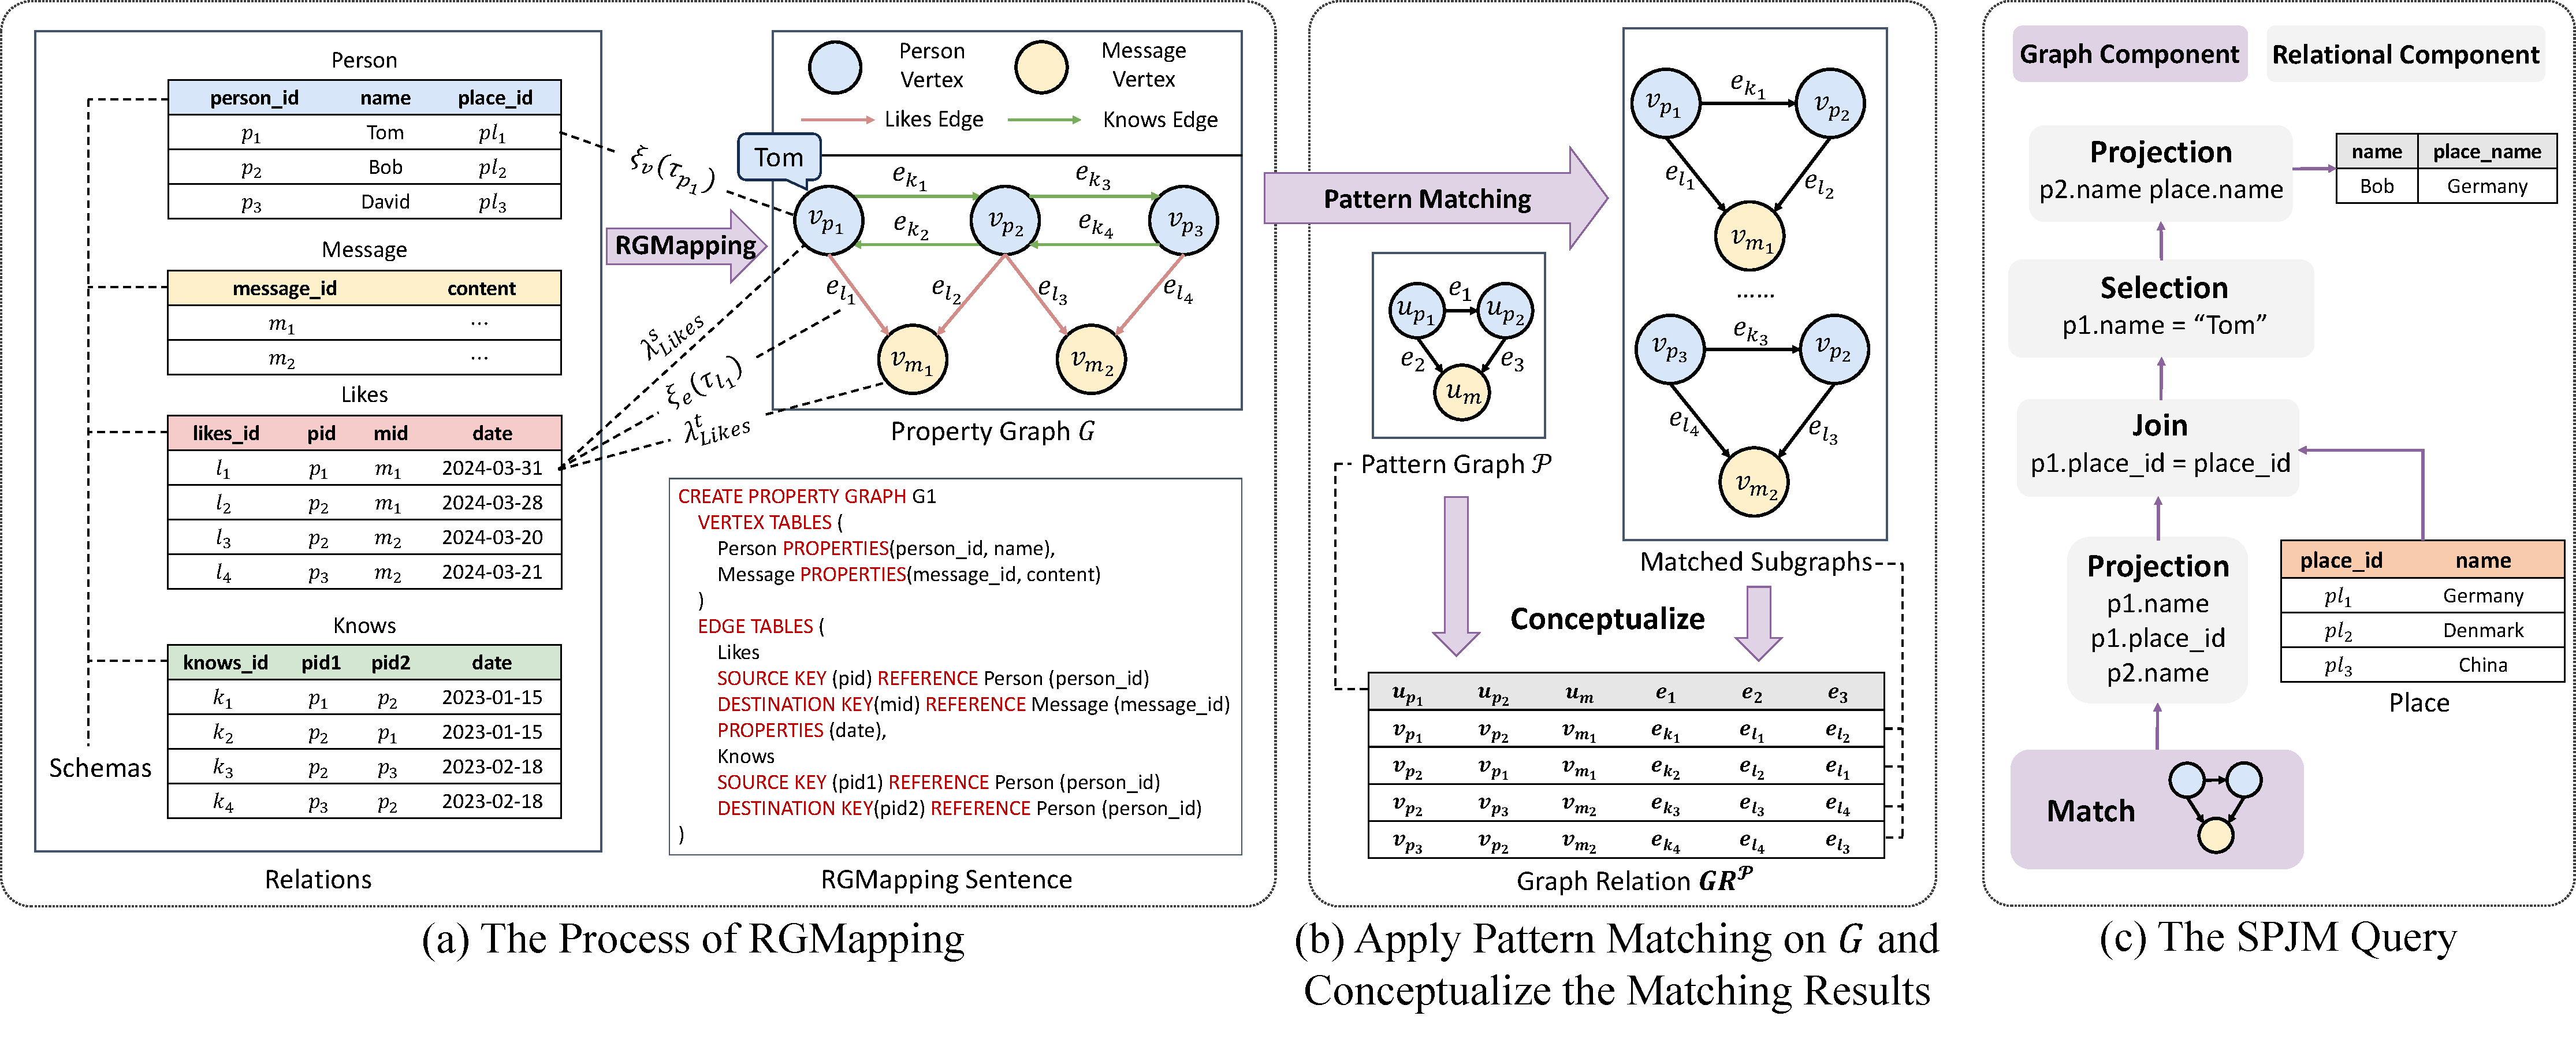
\includegraphics[width=\linewidth]{./figures/rgmapping.pdf}
    \caption{An example of \rgmapping.}
    \label{fig:intro-rgmapping-example}
\end{figure*}

\begin{example}
    \label{ex:rgmapping}
    An \rgmapping can be defined following the grammar of SQL/PGQ with \lstinline{CREATE PROPERTY GRAPH} statements.
    Given five relations, an \rgmapping is defined with the statement shown in Fig.~\ref{fig:intro-rgmapping-example}(a).
    \iffalse
    \begin{equation*}
        \begin{split}
            & \textit{Person = (\underline{person\_id}, name, place\_id)} \\
            & \textit{Message = (\underline{message\_id}, content)} \\
            & \textit{Place = (\underline{place\_id}, pl\_name)} \\
            & \textit{Likes = (\underline{likes\_id}, pid, mid, date)} \\
            & \textit{Knows = (\underline{knows\_id}, pid1, pid2, date)}
        \end{split}
    \end{equation*}
    \fi
    %the following statement defines an \rgmapping (\todo{better plot the statement in Figure 4}):
    \iffalse
    \begin{lstlisting}
CREATE PROPERTY GRAPH G1
    VERTEX TABLES (
       Person PROPERTIES(person_id, name),
       Message PROPERTIES(message_id, content)
    )
    EDGE TABLES (
       Likes
       SOURCE KEY(pid) REFERENCE Person(person_id)
       DESTINATION KEY(mid) REFERENCE Message(message_id)
       PROPERTIES(date),
       Knows
       SOURCE KEY(pid1) REFERENCE Person(person_id)
       DESTINATION KEY(pid2) REFERENCE Person(person_id)
    )
    \end{lstlisting}
    \fi
    The described \rgmapping involves assigning tuples from vertex relations such as $\relation{Person}$ and $\relation{Message}$ to graph vertices. For example, vertex $v_{p_1}$ is associated with the tuple $t_{p_1}$ in $\relation{Person}$, and thus assigned ``Person'' label and named ``Tom''. Edge relations $\relation{Likes}$ and $\relation{Knows}$ correspond to graph edges, with their source and target vertices defined by $\lambda_s$ and $\lambda_t$ mappings. Consider edge $e_{l_1}$, originating from tuple $t_{l_1}$ in $\relation{Likes}$, with source vertex $v_{p_1}$ linked to tuple $t_{p_1}$ via the condition of
    ``$t_{l_1}.pid = t_{p_1}.\text{person\_id}$'', and target vertex $v_{m_1}$ associated with tuple $t_{m_1}$
    via ``$t_{l_1}.mid = t_{m_1}.\text{message\_id}$''. This mapping gives $e_{l_1}$ the label ``Likes'' and the attribute of date ``2024-03-31''.
\end{example}

%In the rest of this paper, let $\mathcal{J}_{GR} = 2^{2^{V \cup E}}$ be the domain of graph relations, $\mathcal{J}_R = 2^{2^{D}}$ be the domain of relations, and $\mathcal{J} = \mathcal{J}_{GR} \cup \mathcal{J}_R$.

\subsection{Matching Operator}
\label{sec:graph-relational-algebra}
%In this work, we extend the conventional relational algebra to equip it with the capability to handle graph pattern matching, which lies at the core of graph query processing, and is also the most fundamental extension in SQL/PGQ~\cite{sqlpgq}.

\comment{
Given a property graph $G(V_G, E_G)$, we let $GR$ denote a graph relation over a schema $S = (v_1, v_2, \ldots, v_n, e_1, e_2, \ldots, e_m)$, where the domain of each $v_i$
is the vertex set $V_G$, and the domain of each $e_j$ is the edge set $E_G$ in $G$, respectively.
}
 %and facilitating a holistic approach to data management and query

Consider a property graph \(G(V_G, E_G)\), alongside a pattern graph\footnote{Throughout this paper, we deal with \emph{connected} pattern graphs for simple presentation, where each vertex is associated with at least one edge.}, represented as \(\pattern(V_\pattern, E_\pattern)\). Here, \(\pattern\) is a property graph that does not possess attributes.
%Graph pattern matching is defined as the task of identifying all subgraphs within a target graph \(G\) that are \emph{homomorphic} to \(\pattern\).
Graph pattern matching seeks to determine all subgraphs in \(G\) that are \emph{homomorphic} to \(\pattern\).
Formally, given a subgraph $g \subseteq G$, a homomorphism from \(\pattern\) to \(g\) is a \emph{surjective}, total mapping \(\sigma: V_\pattern \cup E_\pattern \to V_{g} \cup E_{g}\) that satisfy the following conditions: (1) For every vertex \(v \in V_\pattern\), there is a corresponding vertex \(\sigma(v) \in V_{g}\) with \(\lab_\pattern(v) = \lab_{g}(\sigma(v))\); (2) For each edge \(e = (u_s, u_t) \in E_\pattern\), there is a corresponding edge \(\sigma(e) = (v_s, v_t) \in E_{g}\), ensuring that the mapping preserves the edge's the label, as well as its source and target vertices , that is \(\lab_\pattern(e) = \lab_g(\sigma(e))\), and \(\sigma(u_s) = v_s\), \(\sigma(u_t) = v_t\). It's important to highlight the homomorphism semantics, as one of the widely used semantics for graph pattern matching~\cite{angles2017foundations}, \modify{does} not require each pattern vertex and edge being uniquely mapped to distinct vertices and edges in the data graph. This facilitates a seamless integration between graph pattern matching and relational operations, as will be further discussed in~\reflem{xx}.

The outcomes of graph pattern matching can be succinctly modeled as a relation \(GR_G^\pattern\), or more compactly \(GR^\pattern\) in clear contexts, defined over the schema \(S = V_\pattern \cup E_\pattern\). Here, the sets \(V_G\) and \(E_G\) serve as the respective domains for the vertices and edges identified through the matching process. Within this framework, we refer to such a relation as a \emph{Graph Relation}, a construct where all attributes are derived from the domain of a property graph.
It is essential to recognize that any property graph \(G\) can be conceptualized as a graph relation \(GR^G\), represented by a singular tuple that collectively encompasses all of its vertices and edges. Throughout this paper, we treat the notions of a property graph and a tuple of graph relation as essentially interchangeable terms. In alignment with this perspective, we proceed to elaborate on the \emph{Matching} operator as follows.

%The formulation of graph relation inherently positions any graph $G$ as a graph relation consisting of a single tuple that encapsulates the entirety of its vertices and edges.
%he results of graph pattern matching can be represented as a relation \(R_G(\pattern)\) (or \(GR(\pattern)\) for short when the context is clear) over the schema  \(S = V_\pattern \cup E_\pattern\), wherein \(V_G\) and \(E_G\) act as the domains for the vertices and edges that have been matched, respectively. In this paper, we call such a relation a \emph{graph relation}, when all attributes of the relation are from the domain of a property graph.
%It's clear that any graph $G$ can be represented as a graph relation consisting of a single tuple that encapsulates the entirety of its vertices and edges. In this paper, the concepts of property graph and graph relation can always be used interchangeably. In this context, we introduce the \emph{Match} operator as detailed below.

%likewise expressible as a graph relation \(GR_G(\pattern)\) (or \(GR(\pattern)\) for short when the context is clear) based on the schema \(S = V_\pattern \cup E_\pattern\), wherein \(V_G\) and \(E_G\) act as the domains for the vertices and edges that have been matched, respectively. In this context, we introduce the \emph{Match} operator as detailed below.

\begin{definition}[Matching Operator, \(\matching\)]
    \label{def:matching}
    The Matching Operator, denoted as \(\matching\), is designed to perform graph pattern matching on a given graph relation \(GR\) against a specified pattern graph \(\pattern\). For each graph instance \(g\) within \(GR\), \(\matching\) identifies all subgraphs of \(g\) that are homomorphic to \(\pattern\), and subsequently, aggregates these mappings to construct a comprehensive graph relation. The operation of the matching Operator can be formally articulated as \(\matching(GR, \pattern) = \bigcup_{g \in GR} GR_g^\pattern\).%, where each \(GR_g^\pattern\) represents the subgraph(s) of \(g\) that align with the structure and properties of \(\pattern\).
\end{definition}

\begin{example}
    \label{ex:matching}
    Consider the property graph \(G_1\) derived from the \rgmapping in \refex{rgmapping}. As shown in \reffig{intro-rgmapping-example}(a), we conceptualize the graph as a graph relation \(GR^{G_1}\) that contains a single tuple, encapsulating all vertices and edges in \(G_1\).
    Given a pattern graph \(\pattern\) shown in Fig.~\ref{fig:intro-rgmapping-example}(b), the results of graph pattern matching are subgraphs of \(G_1\) that are homomorphic to \(\pattern\), which are represented as a graph relation \(GR^\pattern = \matching(GR^{G_1}, \pattern)\), wherein each tuple corresponds to one of the matched subgraph.
\end{example}

This definition ensures that the matching operator is inherently closed regarding graph relations,
which adheres to the language opportunities of ``nested matching'' (specified as PGQ-079) in SQL/PGQ~\cite{sql-pgq}.
In this paper, we only handle cases where $G$ represents the entire property graph, and thereafter simplify the matching operator notation to $\matching_G(\pattern)$, or $\matching(\pattern)$ when the context is clear.

\subsection{Problem Definition}
\label{sec:problem-definition}

To study relational query optimization, it is common to focus on a category of queries known as \spj queries,
which encapsulate the three most frequently employed operations in database management: select, project, and (natural) join.
These operations form the backbone of many relational queries. Given a set of relations \(R_1, R_2, \ldots, R_m\),
an \spj query is formally represented as:
\[
Q = \pi_A(\sigma_d(R_1 \Join \cdots \Join R_m)).
\]

Inspired from the \spj paradigm, we introduce a novel category of queries, termed \spjm queries, to address SQL/PGQ~\cite{sql-pgq} queries that
blend relational and graph operations. The \spjm framework augments \spj queries by incorporating a matching operator, thereby enriching the query's expressive power to seamlessly navigate both relational and graph data domains.
Given the set of relations and a property graph \(G\) constructed from these relations via an \rgmapping (\refdef{rgmapping}),
an \spjm query is articulated as:

\begin{equation}
    \label{eq:spjm}
Q = \pi_A(\sigma_d(R_1 \Join \cdots \Join R_m \Join \widetilde{R}))
\end{equation}
where
\[
<<<<<<< HEAD
\widetilde{R} = \widehat{\pi}_{attr*}\matching_G(\pattern).
=======
\widetilde{R} = \widehat{\pi}_{attr}\matching(GR^G, \pattern).
>>>>>>> 3824217fe5fb0d4c78cdad9c08d2218dd405dce8
\]
In this formulation, \(\widehat{\pi}_{attr*}(GR)\) denotes a specialized projection operator to extract attributes (including the id and label)
from vertices and edges within a graph relation $GR$.
This process helps ``flatten'' graph elements into relational tuples.
For example, a vertex represented as \(\{\id=0, \lab=Person, age=18, name=Tom\}\) becomes a tuple of \((0, Person, 18, Tom)\).
In fact, the projection operation is designed to selectively retrieve specific attributes from vertices and edges as required, but for simplicity, we assume that all attributes are extracted if otherwise specified.
The construction makes the resultant relation \(\tilde{R}\) fully compatible with original relational operations.

In this paper, we study the problem of optimizing \spjm queries in \refeq{spjm}.


%\todo{give a final example of spjm}
\begin{figure}
    \centering
    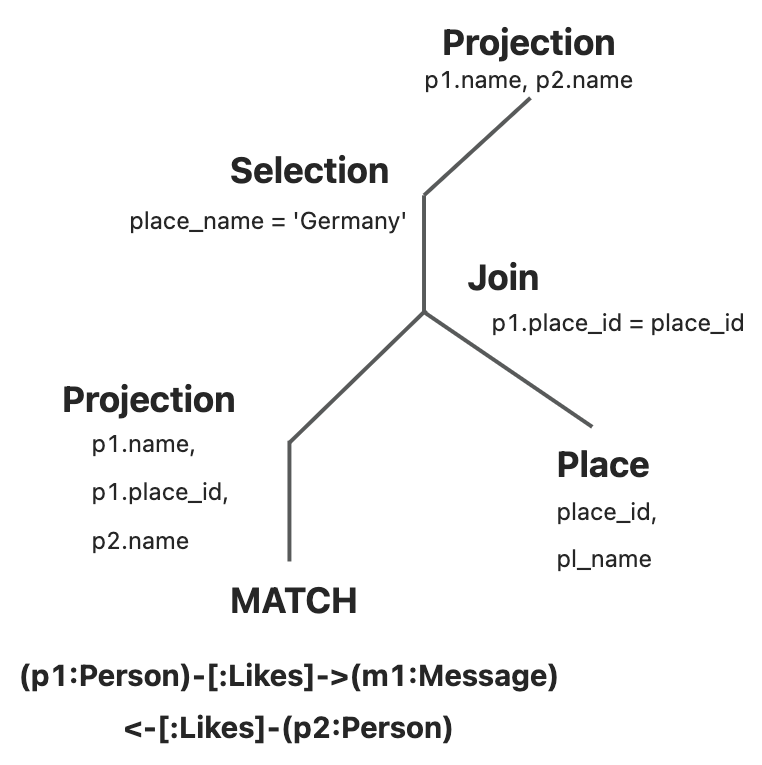
\includegraphics[width=.6\linewidth]{./figures/spjm.png}
    \caption{The operator tree of an SPJM query.}
    \label{fig:spjm}
\end{figure}

\iffalse
\begin{lstlisting}
SELECT f.pn1, f.pn2
FROM GRAPH_TABLE (G1
    MATCH (p1:Person)-[:Likes]->(m1:Message)<-[:Likes]-(p2:Person),
        (p1)-[:Knows]->(p2),
        (p2)-[:Knows]->(p1)
    COLUMNS (
        p1.name as pn1,
        p1.place_id as ppid,
        p2.name as pn2)
) f, Place pl
WHERE f.ppid = pl.place_id
AND pl.pl_name = 'Germany';
\end{lstlisting}
\fi

\begin{example}
    An SPJM query follows the grammar of SQL/PGQ is shown in \reffig{intro-rgmapping-example}(c) and the corresponding query tree is also presented.
    This query aims to find two persons who like the same message and know each other, one of whom lives in Germany.

    According to the query tree, after the results of the match operator are obtained as described in \refex{matching}, a specialized projection operator is applied to extract attritubes from vertices and this operator returns a relational table (i.e., $R_{M}$ in \reffig{intro-rgmapping-example}(c)).
    Next, the join, selection, and projection operators are leveraged in sequence to obtain the final results.
    Specifically, Tom and Bob know each other and like the same message $m_1$.
    Besides, Tom is a Germany.

    \todo{Figure 5 can also be plot in Figure 4. Like rgmapping,
    the query can also be introduced by a SQL/PGQ statement.}
    \comment{
    As shown in \reffig{intro-rgmapping-example}, the property graph $G_1$ obtained from \refex{rgmapping}
    %Since three relations, i.e., \textbf{Person}, \textbf{Message}, and \textbf{Likes}, are utilized as labels of vertices and edges in the pattern graph, an \rgmapping is defined to map them to a property graph.
    %The details are introduced in Example \ref{example:rgmapping}.
    %As property graph \(G1\) is obtained,
    can be conceptualized as graph relation \(GR^{G_1}\), which consists of a single tuple that contain all the vertices and edges in \(G_1\).
    Then, the matching operator is applied on \(GR^{G_1}\) to find subgraphs homomorphic to the pattern graph $\pattern$, which are given as  \(GR^\pattern\) in \reffig{intro-rgmapping-example}.
    %This process is equivalent to performing pattern matching on property graph $G1$.
    The results of pattern matching are those graphs in \(\mathcal{G}\).
    Please note that each graph in \(\mathcal{G}\) corresponds to a row of \(GR^{M}\).

    After that, a specialized projection operator is applied to extract attritubes from vertices and the operator returns a relational table.
    Next, the join, selection, and project operator are leveraged in sequence to obtain the results.
    }
\end{example}

%is a relation generated by projecting the outputs of the matching operator $\mathcal{M}$ to relations of properties.
%Besides, $GR_i$ is the graph relation that contains the data graphs that pattern matching is conducted on and $\mathcal{P}_i$ is the pattern.
%$prop_i$ is a list of necessary properties of vertices and edges in the resultant relation.

\iffalse
Regarding the SPJM problem, the main difference between the aforementioned four types of optimizers lies in their search space when optimizing the physical implementation of the matching operator.
Specifically, for $Rel$ methods, the matching operator is implemented with only joins that do not leverage graph indices (named relational joins) such as hash joins.
Therefore, $\widetilde{R}_i$ can be optimized with the relational optimizer.
For $Rel^+$ methods, in the process of optimization, the matching operator is implemented with relational joins.
Thus, the relational optimizer is also utilized to optimize $\widetilde{R_i}$.
However, after that, relational joins are replaced with joins that leverage graph indices (named graph joins) if possible such as sip join in GrainDB.
For $Rel+G$ methods, graph joins are considered in implementing the matching operator.
Then, operators inside of $\widetilde{R}_i$ are optimized by the graph optimizer, while the operators out of $\widetilde{R}_i$ are optimized by the relational optimizer.
Besides, the optimizations cannot be simultaneously related to operators within and outside of $\widetilde{R}_i$.
For example, the filter operators, i.e., $\sigma_d$ cannot be pushed into $\widetilde{R}_i$.
For $Rel\&G$, such optimizations are allowed.
\fi

% The search space for relgo in the context of a SPJG query consists of operator trees that correspond to sequence of join operators, e.g., the sequence
% \begin{lstlisting}
%     Join(Join(Join(Join(GR_1, GR_2), R_1), R_2), R_3)
% \end{lstlisting}


\iffalse
\subsection{Equivalence Between Graph Pattern Matching and Graph Relational Operators}
\label{sec:proof-gpm-gro}

For the SPJG problem to be solved in this paper, we need to obtain the graph relations by pattern matching.
In detail, the pattern matching process ought to be expressible through the traversal of paths, which are sequences of source, expand, and join operators.
In this section, we prove that the matching operator can be replaced with source, expand, and join operators. without changing the semantics of the query.
Then, the matching order can be further optimized by relgo.

We start from the case that there is only one path in the specified pattern, and firstly, we focus on homomorphic pattern matching.
Then, we have the following theorem.

\begin{theorem}
    Homomorphic pattern matching with a path pattern can be expressed with graph relational algebra expressions.
\end{theorem}
\begin{proof}
    The graph relational algebra operators related to pattern matching include source, expand, join, and extend-intersect.
    Then, we prove the theorem by induction.
    Let each vertex and edge in a path pattern be an element.
    If for each edge in a pattern, its adjacent vertices are also specified in the pattern, then the pattern is called a strict pattern $P$.
    Otherwise, it is a loose pattern $\hat{P}$.

    %Since path patterns specified in SQL/PGQ are all strict patterns are, the induction is conducted on the number of elements in the strict pattern.
    The path pattern is a strict pattern, and induction is conducted on the number of elements in the strict pattern.
    When there is only one element (i.e., a vertex like ``(u:Label)'') in the pattern, the corresponding algebra expression of the pattern is $\bigcirc_{(u:\text{Label})}$, and it is clear that the expression equals the pattern.

    Then, suppose for a path pattern with at most $n$ elements, the corresponding algebra expressions have the same meaning as matching the path pattern.
    Denote a graph relational algebra with the same meaning as matching path pattern $P$ by $E_p$.

    When there are $n + 1$ elements in the path pattern $P$:

    %Condition 1: $P = P_1, P_2$, i.e., pattern $P$ is obtained by concatenating subpatterns $P_1$ and $P_2$.
    %(e.g., $P_1 = (u)-[e]-(v), P_2 = (u)-[e']-(w), P = (u)-[e]-(v), (u)-[e']-(w)$).
    %Then, $E_{p_1} \Join E_{p_2}$ equals $P$, since join operator implemented in relational databases follows the semantics of homomorphism.


    Condition 1: $P = P_1 - \hat{P}_2$.
    Without loss of generality, suppose vertex $v$ in $P_1$ is adjacent to an edge in $P_2$.
    (e.g., $P_1 = (u)-[e]-(v), P_2 = [e']-(w), P = (u)-[e]-(v)-[e']-(w)$).
    Then, let $P_3 = (v)-\hat{P}_2$, and the corrsponding algebra expression of $P$ can be $E_{p_1} \Join E_{p_3}$.
    $E_{p_1} \Join E_{p_3}$ equals $P$, since join operator implemented in relational databases follows the semantics of homomorphism.
    Moreover, if $\hat{P}_2$ only consists of one vertex and an edge adjacent to it (i.e., $\hat{P}_2 = [e:eLabel]-(v_t:vLabel)$).
    Then, the corresponding algebra expression of $P$ can also be $\updownarrow_{(v)}^{(v_t:vLabel)}[e:eLabel]E_{p_1}$.
    The expand operator is also implemented by joining relational tables, which follows the semantics of homomorphism.

    Condition 2: $P = P_1$ extends $v$ through edges $[e_1:eLabel1], \cdots [e_k:eLabelk]$ ($k \geq 1$), i.e., at least one vertex in $P_1$ connects to vertex $v$.
    Then, the corresponding algebra expression of $P$ is
    \begin{equation*}
        E_{p_1} \Diamond_{v_1, \cdots, v_k}^{eLabel1, \cdots, eLabelk} \bigcirc_{(v:vLabel)}.
    \end{equation*}
    Since the extend-intersect operator is implemented with relational joins and follows the semantics of homomorphism, the algebra expression has the same meaning as matching the path pattern.

    In conclusion, the corresponding algebra expressions of path pattern $P$ with $n + 1$ elements have the same meaning as matching the path pattern.

    In conclusion, adopting the homomorphism semantics, matching path patterns has the same meaning as the corresponding graph relational algebra expressions.
\end{proof}

When the match operator adopt the isomorphic semantics, it is straightforward to add some constraints with selection operators to get the graph relational expressions equal to the match operator.
Furthermore, when there are more than one path specified in the pattern, the expressions for different paths can be connected with join operators and the obtained expressions equal to the match operator.


Besides the WALK mode by default, when the path patterns are in TRAIL, ACYCLIC, or SIMPLE mode, we still have the same conclusions.
Specifically, in TRAIL, ACYCLIC, or SIMPLE mode, a selection operator needs to be added to remove the results with repeated edges or vertices.
In detail, the selection operator should wrap the corresponding algebra expression of path patterns in the WALK mode.
For example, in the TRAIL mode, the corresponding graph relational algebra expression of $P = P_1 - P_2$ is $\sigma_{c}(E_{p_1} \Join E_{p_2})$ or $\sigma_{c}(\updownarrow_{(v)}^{(v_t:vLabel)}[e:eLabel]E_{p_1})$, where $c$ is the condition specifying that every two different pattern edges bind to different edges in each result.
In the ACYCLIC and SIMPLE mode, condition $c$ should be specified according to the constraints of the mode.

Furthermore, there may be more than one path patterns specified in the <Pattern> part of SQL/PGQ queries, and the different path patterns may have different path modes.
Denote the path patterns by $P_1, \cdots, P_k$.
According to SQL/PGQ, the binding results of different path patterns are joined together.
If the match mode in SQL/PGQ is set to \textbf{REPEATABLE ELEMENTS}, there is no more constraint, and ``MATCH $P_1, \cdots, P_k$'' has the same meaning as $P_1 \Join \cdots \Join P_k$, both of which have the semantics of homomorphism.
Otherwise, if the match mode in SQL/PGQ is set to \textbf{DIFFERENT EDGES}, the same edge cannot bind to different variables in different path patterns.
Therefore, a selection operator is needed, and ``MATCH $P_1, \cdots, P_k$'' has the same meaning as $\sigma_{d}(P_1 \Join \cdots \Join P_k)$, where $d$ is the condition specifying that each edge cannot bind to more than one variables across all path patterns.
\fi
